\documentclass{article}

% General physics constructs
\newcommand{\bra}[1]{\langle #1 |}
\newcommand{\ket}[1]{| #1 \rangle }
\newcommand{\braket}[2]{\langle #1|#2\rangle}
\newcommand{\bbraket}[3]{ \langle #1 | #2 | #3 \rangle }
\newcommand{\boltzmann}{k_b}

% Common math
\newcommand{\norm}[1]{\left \lvert #1 \right \rvert}
\newcommand{\abs}[1]{\left \lvert #1 \right \rvert}  % These two are redundant. Consider removing one.

\newcommand{\avg}[1]{\left \langle #1 \right \rangle}  % Should get rid of this, as "average" isn't specific.
\newcommand{\angavg}[1]{\left \langle #1 \right \rangle}

\newcommand{\VS}{\textit{\textbf{V}}}
\newcommand{\Tr}{\textrm{Tr}}
\renewcommand{\Re}{\textrm{Re}}
\renewcommand{\Im}{\textrm{Im}}
\newcommand{\basis}[1]{\{\ket{#1}\}}

% Quantum
\newcommand{\nboseeinstein}{n_\text{BE}}
\newcommand{\gammaup}{\Gamma_\uparrow}
\newcommand{\gammadown}{\Gamma_\downarrow}
\newcommand{\gammaupdown}{\Gamma_{\uparrow \downarrow}}
\newcommand{\gammaemission}{\Gamma_\text{loss}}
\newcommand{\qualityfactoremission}{Q_{d,\text{loss}}}

% Qubits
\newcommand{\omegaqubit}{\omega_{10}}

% Circuits
\newcommand{\impedance}{Z_0}
\newcommand{\resistorsource}{R_s}
\newcommand{\vsource}{V_s}
\newcommand{\vsourcerms}{V_{s,\text{rms}}}
\newcommand{\vloadrms}{V_{l,\text{rms}}}

% Signals and noise
\newcommand{\psdsingle}{S_\text{ss}}
\newcommand{\psddouble}{S_\text{ds}}
\newcommand{\noiseavailable}{S_{p,a}^e}
\newcommand{\spectralengineer}{S^e}
\newcommand{\spectralsymmetric}{S^\text{symm}}
\newcommand{\spectralattenuator}{\spectralengineer_{\poweravailable, \text{att.}}}

% Microwaves
\newcommand{\vright}{V_+}
\newcommand{\vleft}{V_-}
\newcommand{\iright}{I_+}
\newcommand{\ileft}{I_-}
\newcommand{\poweravailable}{P_a}

% Figures. Example usage:
% \quickfig{\columnwidth}{my_image}{This is the caption}{fig:my_fig}
\DeclareRobustCommand{\quickfig}[4]{
\begin{figure}
\begin{centering}
\includegraphics[width=#1]{#2}
\par\end{centering}
\caption{#3}
\label{#4}
\end{figure}
}

\DeclareRobustCommand{\quickwidefig}[4]{
\begin{figure*}[h]
\begin{centering}
\includegraphics[width=#1]{#2}
\par\end{centering}
\caption{#3}
\label{#4}
\end{figure*}
}

\DeclareRobustCommand{\quickfigcentered}[4]{
  \begin{figure}
  \makebox[\textwidth][c]{\includegraphics[width=#1]{#2}}
  \caption{#3}
  \label{#4}
  \end{figure}
}

%Packages
\usepackage{amsmath}
\usepackage{amstext}
\usepackage{amssymb}
\usepackage{appendix}
\usepackage{coseoul}
\usepackage{graphicx}
\usepackage{import}
\usepackage{lscape}
\usepackage{modular}

\usepackage[pdfpagemode=UseNone,pdfstartview=FitH,colorlinks=true,linkcolor=blue,citecolor=blue,urlcolor=blue]{hyperref}
\usepackage[all]{hypcap}


\newcommand{\citeinternaltype}{Ref.\,}
\newcommand{\Citeinternaltype}{Reference}
\newcommand{\citeinternalref}[1]{\cite{Sank:#1}}


%\author{Daniel Sank \\ \small{Google Quantum AI \\ Formerly Department of Physics, UCSB}}
\title{Quantum Harmonic Oscillator}
\date{16, October 2008}

\begin{document}

\maketitle

Here I collect useful formulae regarding the quantum simple harmonic oscillator.
The idea is to provide expressions for things like matrix elements and zero point fluctuations in terms of generalized Hamiltonian parameters so that they can easily be applied to any harmonic system.

\levelstay{DFT basics}

From the strictly mathematical point of view a series of experimental data is characterized by only one parameter, the number of points in the time series, which we denote by $N$.
Any mathematical formulae we develop should involve only this one parameter.

\leveldown{Definition}

Consider a time series of data written as $x(n)$ where $n \in [0,\dots,N-1]$ labels the discrete time axis.
The DFT, like all Fourier transforms, is based on the fact that $x(n)$ can be written as a sum of exponentials,
\begin{equation}
x(n)=\frac{1}{N}\sum_{k=0}^{N-1}X(k)\, e^{i2\pi nk/N} \label{eq:iDFT_def}
\end{equation}
where the complex weights $X(k)$ are given by
\begin{equation}
X(k)=\sum_{n=0}^{N-1}x(n)\, e^{-i2\pi nk/N} \label{eq:DFT_def}
\end{equation}
These formulae can be shown to be consistent by substituting (\ref{eq:DFT_def}) into  into (\ref{eq:iDFT_def}).
The indices $n$ and $k$ run from $0$ to $N-1$ which we call the \textbf{baseband}.
The pair of equations (\ref{eq:iDFT_def}) and (\ref{eq:DFT_def}) are not the only way to define the DFT.
The only requirements are that the product of the prefactors of the two sums is $1/N$ and the signs of the exponentials are opposite.
Our choice to to put the factor of $1/N$ in the first equation matches the choice made in numpy and Matlab.
The various numerical packages in various programming languages use different conventions, so make sure to always check this before writing a program using any particular DFT.
Formulas given below assume the DFT specified by equations (\ref{eq:iDFT_def}) and (\ref{eq:DFT_def}), but the appropriate modifications of these for various DFT conventions should be clear once you understand the present case.


\levelstay{General Properties}

Here we list the most important properties of the DFT.

\leveldown{Fourier frequencies}

From equation (\ref{eq:iDFT_def}) we see that our signal $x(n)$ is built up of exponentials $\exp(i2\pi nk/N)$.
We call the frequency $k/N$ the $k^{th}\textbf{ Fourier frequency}$.
The minimum Fourier frequency is 0 and the greatest is $(N-1)/N\approx1$.
These frequencies are in ``index units,'' meaning that the exponential $\exp(i 2 \pi n k / N)$ goes through $k/N$ oscillations per step of the index $n$.
Note that a Fourier frequency of 1 (which is \emph{not} in the baseband) is actually just a constant function; if the signal goes through exactly one cycle per index, it attains the same value at each index.


\levelstay{All information in baseband}

A signal $x(n)$ is completely determined by knowledge of $X(k)$ for $k$ in the baseband $[0,\ldots,N-1]$.
Still, if we have a series $x(n)$ in hand and we regard equation (\ref{eq:DFT_def}) as a formula that spits out $X(k)$ for $\emph{any}$ integer $k$, we can compute $X(k)$ for $k$ outside the baseband.
However, these new $X(k)$'s are not independent of the ones in the baseband.
To see this, first note that any integer $k$ can be written as $k=p+mN$ where $p \in [0..N-1]$ and $m$ is an integer, as shown in Figure \ref{fig:baseband}.
Note that if $m=0$ then $k=p$ and $k$ is in the baseband, and if $m \neq 0$ then $k$ is not in the baseband.
Computing the DFT we find
\begin{align}
X(k) &= \sum_{n=0}^{N-1} x(n) e^{-i2\pi nk/N}\\
&= \sum_{n=0}^{N-1} x(n) e^{-i2\pi np/N} e^{-i2\pi nm} \\
&= \sum_{n=0}^{N-1} x(n)e^{-i2\pi np/N} \\
&= X(p) \, .
\end{align}
The DFT computed for $k$ is exactly equal to the DFT computed for $p$.
This means that, given a series $x(n)$, only the weights $X(k)$ are uniquely determined only for $k \in [0, \ldots , N-1]$.
In other words, all of the information about the original series $x(n)$ is contained in the set $X(k)$ for $k$ in the baseband.
Fourier coefficients can be computed for $k$ outside this range, but they are all related to the ones in the baseband by translation in $k$ space:
\begin{equation}
X(k) = X(k+mN) \quad \textrm{for all integers }m \, . \label{eq:translational_symmetry}
\end{equation}

\begin{figure*}[t]
\begin{centering}
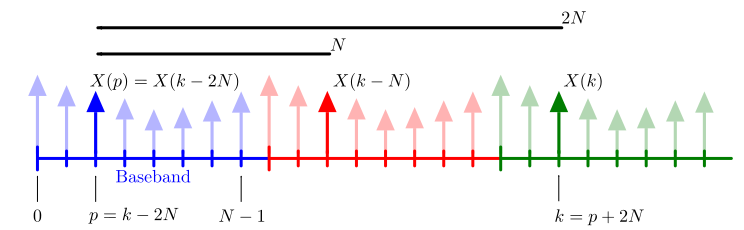
\includegraphics[width=\textwidth]{baseband.pdf}
\par\end{centering}
\caption{Illustration of the baseband and higher bands.}
\label{fig:baseband}
\end{figure*}


\levelstay{DFT of a baseband complex exponential}

The DFT of an exponential is of fundamental importance.
Given a signal $x(n)=\exp(i2\pi nq/N)$ with $q$ in the baseband, the DFT value at a frequency $k$ in the baseband is
\begin{align}
  X(k) =& \sum_{n=0}^{N-1} e^{i2\pi nq/N}e^{-i2\pi nk/N} \\
  =& N \delta_{k, q} \, .
\end{align}
Of course, as already discussed, the DFT value for $k$'s outside the baseband are uniquely determined by those in the baseband.
In particular, in this case we have
\begin{equation}
  X(k + mN) = N \delta_{k, q} \, .
\end{equation}
This is a series of delta peaks separated from each other by $N$ units in frequency space.
Note that this agrees with our previous discussion which said that all DFT coefficients separated by $N$ must be equal.
As previously explained, it makes sense to ignore the coefficients for $k$ outside the baseband, in which case the DFT of the exponential becomes
\begin{equation}
X(k) = \delta_{k,p} \label{eq:dftExponential}
\end{equation}
where $p$ is the \emph{unique} integer in the baseband which is related to $q$ by translation by an integer multiple of $N$, ie. $p=q-mN$.

\levelstay{Aliasing}

What happens if we have an exponential signal $x(n)=e^{i2\pi nq/N}$ when $q$ is outside the baseband?
According to (\ref{eq:dftExponential}) we get a delta peak $\delta_{k,p}$ with $p$ in the baseband and $p = q-mN$ for some integer $m$.
The value of $m$ doesn't matter, the point is that an exponential at a frequency $q$ outside the baseband has the same DFT as an exponential with Fourier frequency $p$ inside the baseband.
A consequence is that if you measure a signal $A\exp\left[i2\pi nq/N\right]+B\exp\left[i2\pi n(q+mN)/N\right]$ the DFT will look exactly the same as if you had measured $(A+B)\exp\left[i2\pi nq/N\right]$.
The indistinguishability of these signals is called $\textbf{aliasing}$, because the actual signal at higher frequency $q+mN$ \emph{looks} like the lower frequency $q$ in frequency space.
What's going on here is that signals with Fourier frequency outside the baseband oscillate more than once per data point, but since we only sample once per data point these oscillations are hidden and the DFT sees the signal at a lower frequency.

In calculations it can be annoying to replace $q$ values outside the baseband by $p+mN$ explicitly.
Instead, you can just do the replacement once the computation is complete.
To get this right use the following \textbf{rules for computing DFTs}
\begin{equation}
  \left[ \textrm{DFT}\left( e^{i2\pi nq/N} \right)\right](k) = \delta_{k,q} \, .
\end{equation}
Then, if $q$ is outside the baseband, at the end of the calculation find the corresponding $p$ inside the baseband and make the replacement
\begin{equation}
  \delta_{k,q} \rightarrow \delta_{k,p} \quad q=p+mN \, . \label{eq:aliasReplacement}
  \, .
\end{equation}

\section{Coherent States}

Suppose we want to find an eigenvector of the lowering operator. For starters we know that the state $\ket{0}$ is an eigenket of the lowering operator with eigenvalue $0$. We also know that to translate $a$ by an amount $\phi$ we should apply the operator $\exp[\phi a^{\dagger}]$. Therefore we guess that the general eigenket of $a$ is \begin{equation}
\ket{\phi}=e^{\phi a^{\dagger}}\ket{0} \end{equation}
With this definition we have, \begin{eqnarray*}
a\ket{\phi} & = & a\exp[\phi a^{\dagger}]\ket{0}\\
& = & \sum_{n=1}^{\infty}\frac{\phi^{n}}{n!}a(a^{\dagger})^{n}~\ket{0}\end{eqnarray*}
Note that since $[a,(a^{\dagger})^{n}]=n(a^{\dagger})^{n-1}$ we have \begin{equation}
a(a^{\dagger})^{n}=(a^{\dagger})^{n}a+n(a^{\dagger})^{n-1} \end{equation}
So then \begin{equation}
a\ket{\phi}=\sum_{n=1}^{\infty}\frac{\phi^{n}}{n!}[(a^{\dagger})^{n}a+n(a^{\dagger})^{n-1}]~\ket{0} \end{equation}
And since $a\ket{0}=0$ we can drop the $(a^{\dagger})^{n}a$ term, leaving, \begin{eqnarray*}
a\ket{\phi} & = & \sum_{n=1}^{\infty}\frac{\phi^{n}}{n!}[n(a^{\dagger})^{n-1}]~\ket{0}\\
& = & \phi~\sum_{n=1}^{\infty}\frac{\phi^{n-1}}{(n-1)!}(a^{\dagger})^{n-1}~\ket{0}\\
a\ket{\phi} & = & \phi\ket{\phi}\end{eqnarray*}
So the kets $\ket{\phi}$ are eigenkets of $a$ as we hoped.
HOWEVER, we have not checked normalization...
XXX Check normalization.

Another useful property is that \begin{eqnarray*}
\partial_{\phi}\ket{\phi} & = & \sum_{n=1}^{\infty}\frac{n\phi^{n-1}}{n!}(a^{\dagger})^{n}~\ket{0} \\
& = & \sum_{n=1}^{\infty}\frac{\phi^{n-1}}{(n-1)!}a^{\dagger}(a^{\dagger})^{n-1}~\ket{0}\\
\partial_{\phi}\ket{\phi} & = & a^{\dagger}\ket{\phi}\end{eqnarray*}


A very important identity that is used in the context of Wigner functions
is \begin{equation}
\int\frac{d\Re(\phi)d\Im(\phi)}{\pi}e^{-\phi^{*}\phi}\ket{\phi}\bra{\phi} \end{equation}


\levelstay{Driven Oscillator}

Coherent states exist in nature because a classical harmonic drive applied to a harmonic oscillator system results in a coherent state.
Consider the energy associated with application of a spatially uniform force field: energy = -force $\times$ distance.
Therefore, the Hamiltonian term associated with this force is
\begin{equation*}
  H_{\textrm{drive}}
  = -x F(t)
  = -(a + a^\dagger) f_x(t)
\end{equation*}
where $f_{x} = x_\text{zpf} F(t)$ has dimensions of energy.
This kind of driving is called a ``linear'' or ``dipole'' drive.
We can, for free, add a term proportional to the conjugate variable:
\begin{align*}
  H_{\textrm{drive}}
  &=  -(a+a^{\dagger})f_{x}(t)-(-i)(a-a^{\dagger})f_{y}(t)\\
  &= a(-f_{x}+if_{y})+a^{\dagger}(-f_{x}-if_{y})
\end{align*}
and define
\begin{equation}
  f(t) = -f_x(t) + i f_y(t)
\end{equation}
so that the drive Hamiltonian is
\begin{equation*}
  H_{\textrm{drive}} = af(t)+a^{\dagger}f(t)^{*} \, .
\end{equation*}
The full Hamiltonian in the Schrodinger picture is
\begin{equation}
  H_S(t)
  = \hbar \omega_0 \left( a^{\dagger} a + \frac{1}{2} \right) + f(t) a(t) + f^*(t) a^\dagger(t)
  \, .
\end{equation}

\leveldown{Solution in the Heisenberg picture}

In this section we solve the driven oscillator problem in the Heisenberg.
We follow the approach in Merzbacher, starting at page 335.
The Hamiltonian in the Heisenberg picture is
\begin{equation}
  H_H(t)
  = \hbar \omega_0 \left( a_H^{\dagger}(t)a_H(t) + \frac{1}{2} \right) + f(t)a_H(t) + f^{*}(t)a_H^{\dagger}(t)
  \, .
\end{equation}
For the rest of this section, we drop the subscript $H$'s and denote $a_H(t) = a(t)$.
Heisenberg's equation of motion for $a(t)$ is
\begin{align*}
  i\hbar\dot{a}(t)
  &= \left[ a(t), H(t) \right] \\
  &= \frac{\partial H(t)}{\partial a^{\dagger}(t)} \\
  &= \hbar\omega_0 a(t) + f^{*}(t) \\
  \textrm{or} \qquad
  \left(d_{t}+i\omega_0\right)a(t) &= -\frac{i}{\hbar}f^{*}(t)
  \, .
\end{align*}
Note that this equation of motion is \emph{exactly} the same as the classical equation of motion for the resonator's action-angle variable (also called ``mode amplitude'' and a variety of other names).
That's one of the points of the Heisenberg picture: we solve for time dependence of the dynamical variables, just as we do in classical mechanics, instead of solving for the time dependence of the mysterios wave function.
The homogeneous solution, i.e. when $f(t) = 0$, is
\begin{equation}
  a_\text{hom.}(t) = a(0) \exp(-i \omega_0 t) \, .
\end{equation}
For the inhomogenous part, we convert to the frequency domain using the Fourier transform convention
\begin{equation}
  f(t) = \int e^{i\omega t} \tilde{f}(t) \frac{d\omega}{2\pi}
  \, .
\end{equation}
The equation for the Green's function can then be rewritten as
\begin{align*}
  \left(d_{t} + i \omega_0 \right) \ket{G_{t_0}}
  =& -\frac{i}{\hbar} \ket{\delta_{t_0}} \\
  \int \left(d_{t} + i \omega_0 \right) \ket{\omega} \braket{\omega}{G_{t_0}} \frac{d\omega}{2\pi}
  =& -\frac{i}{\hbar} \int \ket{\omega}\braket{\omega}{\delta_{t_0}} \frac{d\omega}{2\pi} \\
  \int i\left(\omega + \omega_0 \right) \tilde{G}_{t_0}(\omega) \ket{\omega} \frac{d\omega}{2\pi}
  =& -\frac{i}{\hbar} \int \ket{\omega} e^{-i\omega t_0} \frac{d\omega}{2\pi} \\
  \left(\omega + \omega_0 \right) \tilde{G}_{t_0}(\omega)
  =& -\frac{1}{\hbar} e^{-i\omega t_0} \\
  \tilde{G}_{t_0}(\omega)
  =& -\frac{1}{\hbar \left( \omega + \omega_0 \right)} e^{-i \omega t_0} \\
  G_{t_0}(t)
  =& -\int_{-\infty}^{\infty}\frac{e^{i\omega(t - t_0)}}{\hbar \left(\omega + \omega_0 \right)}\frac{d\omega}{2\pi}
  \, .
\end{align*}
There's a pole on the real line which means we have to impose damping to get a sensible result. We want the $\emph{retarded}$ Green's function to be zero if $t<t_0$ which means we want the poles to exist only when the imaginary part of $\omega$ is in the upper half plane. Therefore we add to the denominator a term $-i\epsilon$,
\begin{align*}
  G_{t_0}^{R}(t)
  =& -\int_{-\infty}^{\infty} \frac{e^{i\omega(t - t_0)}}{\hbar \left(\omega + \omega_0 -i \epsilon\right)} \frac{d\omega}{2\pi} \\
  =& -i \left( 2\pi \right) \frac{1}{\hbar 2\pi} e^{i(-\omega_0 + i \epsilon)(t - t_0)} \Theta(t-t_0) \\
  =& -\frac{i}{\hbar} e^{-i\omega_0(t - t_0)} \Theta(t - t_0)
  \, .
\end{align*}
You can check that the advanced Green's function, which you get by using $+i\epsilon$, is
\begin{equation}
  G_{t_0}^{A}(t) = \frac{i}{\hbar} e^{-i\omega_0 (t - t_0)} \Theta(t_0 - t)
  \, .
\end{equation}
Using the retarded Green's function, we can write the inhomogenious part of the solution as
\begin{align*}
  a_\text{inhom.}(t)
  &= \int_{-\infty}^{\infty}G_{t'}^{R}(t)f^{*}(t')dt' \\
  &= -\frac{i}{\hbar}\int_{-\infty}^{t}e^{-i\omega_0(t-t')}f^{*}(t')dt'
\end{align*}
Note that the retarded Green's function has the effect of including influence from the driving force at times $t'$ only earlier than the evaluation time $t$.
In words: the system is affected only by influences from the past.

Consider the case that the driving force turns on at $t_1$.
We can then write the full solution (homogeneous plus inhomogeneous) for $t > t_1$ as
\begin{equation}
  a(t)
  = a(t_1) e^{-i\omega_0(t - t_1)} \underbrace{- \frac{i}{\hbar} \int_{t_1}^t e^{-i \omega_0(t - t')} f^{*}(t') \, dt'}_{\zeta(t)} \, .
\end{equation}
This relation shows explicitly that during the driving period $a$ acquires the usual $e^{-i\omega_0(t - t_1)}$ dynamical phase from free oscillation, plus an added effect, namely the Fourier transform, of the driving.

\leveldown{Evolution of a coherent state}

We can now show that a coherent state, subject to driving, remains a coherent state.
If the system is in coherent state $\ket{\phi}$ at time $t=0$, then $a\ket{\Psi(0)} = \phi \ket{\Psi(0)}$, and we compute
\begin{align*}
  a \ket{\Psi(t)}
  &= a T_S(t) \ket{\Psi(0)} \\
  &= T_S(t) \underbrace{\left( T_S^\dagger(t) a T_S(t) \right)}_{a(t)} \ket{\Psi(0)} \\
  &= T_S(t) \left( a e^{-i \omega_0 t} + \zeta(t) \right) \ket{\Psi(0)} \\
  &= \left( \phi e^{-i \omega_0 t} + \zeta(t) \right) T_S(t) \ket{\Psi(0)} \\
  &= \left( \phi e^{-i \omega_0 t} + \zeta(t) \right) \ket{\Psi(t)} \\
\end{align*}
which shows that under the effect of driving, a coherent state evolves as
\begin{equation}
  \ket{\phi} \Rightarrow \ket{\phi e^{-i \omega_0 t} + \zeta(t)}
  \, .
\end{equation}

\levelup{Solution in a rotating frame}

In the Heisenberg picture, the equation of motion for the lowering operator was
\begin{equation*}
  \left( d_t + i \omega_0 \right) a(t) = -\frac{i}{\hbar} f^*(t)
  \, .
\end{equation*}
This equation involves two potentially large frequencies: the resonance frequency $\omega_0$ of the oscillator, and the time dependence $f^*(t)$.
In the typical case where the spectral content of $f^*$ is centered near $\omega_0$, we can use the rotating frame to remove the fast time dependence.
Consider the rotating frame defined by
\begin{equation*}
  R(t) = \exp(i \omega_R \, t \, n)
\end{equation*}
which implies $\tilde{H}_S = \hbar \omega_R n$.
The equation of motion for $a_R(t)$ is
\begin{align*}
  i \hbar \dot{a}_R(t)
  &= \left[ a, \tilde{H}_S \right]_R \\
  &= \left(
    \frac{\partial}{\partial a^\dagger} \left( \hbar \omega_R a^\dagger a \right)
    \right)_R \\
  &= \hbar \omega_R a_R(t) \\
  \dot{a}_R(t)
  &= -i \omega_R a_R(t)
\end{align*}
with solution $a_R(t) = \exp(-i \omega_R t) a$.
Meanwhile, the kets evolve in time according to the rotating frame Hamiltonian
\begin{align}
  H_R(t)
  &= i \hbar \dot{R}(t) R^\dagger(t) + R(t) H_S(t) R^\dagger(t) \nonumber \\
  &= \hbar \Delta \, n + \frac{1}{2} \hbar \omega_0 + f(t) a_R(t) + f^*(t) a_R^\dagger(t)
  \label{eq:rotating_frame_hamiltonian}
\end{align}
where $\Delta \equiv \omega_0 - \omega_R$ and we dropped the subscript on $n$ because $n_R(t) = n$.
Since we already solved for $a_R(t)$, it remains only to solve the Schrodinger equation for $H_R(t)$, and then we would be able to find all matrix elements of interest.
However, it's more convenient to take the point of view that Eq.~(\ref{eq:rotating_frame_hamiltonian}) itself is a Schrodinger equation whos matrix elements can be found in the Heisenberg picture.
We can do this by lumping the time dependence of $a_R(t)$ into the drive terms, re-expressing the Hamiltonian as
\begin{equation}
  H_R(t) = \hbar \Delta n + \frac{1}{2}\hbar \omega_0 + f(t)e^{-i \omega_R t} a + f^*(t) e^{i \omega_r t} a^\dagger
\end{equation}
which looks just like the Hamiltonian in the Schrodinger picture (here we write $a$ instead of $a_S$), but with modified time dependence in the drive.
Formally, this Hamiltonian has a propagator $T_R$, and to solve for the time dependence of the kets we'd have to compute $T_R$.
But of course, we can apply the Heisenberg picture to \emph{this} Hamiltonian instead.
Formally, and matrix element can be computed as
\begin{align*}
  \bbraket{\Psi_S(t)}{\mathcal{O}_S}{\Phi_S(t)}
  &= \bbraket{\Psi_R(t)}{R(t) \mathcal{O}_S R^\dagger(t)}{\Phi_R(t)} \\
  &= \bbraket{\Psi_R(0)}{T_R^\dagger(t) R(t) \mathcal{O}_S R^\dagger(t) T_R(t)}{\Phi_R(0)}
  \, .
\end{align*}
In the present case, we have $R(t) a R^\dagger(t) = \exp(-i \omega_R t) a$, and of course $\ket{\Psi_R(0} = \ket{\Psi_S(0)}$, so
\begin{align*}
  \bbraket{\Psi_S(t)}{\mathcal{O}_S}{\Phi_S(t)}
  &= \exp(-i \omega_R t) \bbraket{\Psi_S(0)}{T_R^\dagger(t) a T_R(t)}{\Phi_S(0)}
  \, .
\end{align*}
Therefore, to find matrix elements, we can solve the Heisenberg equation for $a(t)$ with respect to $H_R$, and add the time dependent phase $\exp(-i \omega_R t)$ arising from the rotating frame to that result.
The form of $H_R(t)$ is exactly the same as $H_S(t)$ with the modifications $\omega_0 \rightarrow \Delta$ and $f(t) \rightarrow f(t) e^{-i \omega_R t}$, so the equation of motion is
\begin{equation}
  (d_t + i \Delta) a(t) = - \frac{i}{\hbar} f^*(t) e^{i \omega_R t}
\end{equation}
and the solution for $a(t)$, in the case that the drive turns on at time $t_1$ is
\begin{equation}
  a(t) = a(t_1) e^{-i \Delta (t - t_1)}
  \underbrace{- \frac{i}{\hbar} \int_{t_1}^t e^{-i \Delta (t - t')} f^*(t') e^{i \omega_R t'} \, dt'}_{\zeta_R(t)}
  \, .
\end{equation}
Now we come to the main advantage of the rotating frame.
If the complex function $f(t)$ has spectral weight over a limited band centered at frequency $\omega_d$, then it can be written as $f(t) = \varepsilon(t) \exp(i \omega_t t)$ where $\varepsilon(t)$ has a limited bandwidth.
If we take our rotating frame frequency $\omega_R = \omega_d$, then our equation of motion is
\begin{equation}
  \left( d_t + i \Delta \right) a(t) = - \frac{i}{\hbar} \varepsilon^*(t)
  \, .
\end{equation}
The point of this is that $\Delta = \omega_0 - \omega_d$ and $\varepsilon(t)$ are both slow, so numerics, plots, etc. are easier to understand.

\leveldown{Evolution of a coherent state}

Suppose the state at $t=0$ is a coherent state $\ket{\Psi_S(0)} = \ket{\phi}$.
Then
\begin{align*}
  a \ket{\Psi_S(t)}
  &= a R^\dagger(t) \ket{\Psi_R(t)} \\
  &= a R^\dagger(t) T_R(t) \ket{\Psi_R(0)} \\
  &= R^\dagger(t) \underbrace{R(t) a R^\dagger(t)}_{\exp(-i \omega_R t) a} T_R(t) \ket{\Psi_R(0)} \\
  &= e^{-i \omega_R t} R^\dagger(t) T_R(t) \left(T^\dagger(t) a T_R(t) \right) \ket{\Psi_R(0)} \\
  &= e^{-i \omega_R t} R^\dagger(t) T_R(t) \left(a e^{-i \Delta t} + \zeta_R(t) \right) \ket{\Psi_R(0)} \\
  &= e^{-i \omega_R t} R^\dagger(t) T_R(t) \left(\phi e^{-i \Delta t} + \zeta_R(t) \right) \ket{\Psi_R(0)} \\
  &= \left(\phi e^{-i \omega_0 t} + e^{-i \omega_R t} \zeta_R(t) \right) \ket{\Psi_S(t)} \\
  &= \left(\phi e^{-i \omega_0 t} + \zeta(t) \right) \ket{\Psi_S(t)}
\end{align*}
which is identical to our result in the Heisenberg picture.
So once again we have shown that under the effect of driving, a coherent state remains a coherent state, and the eigenvalue of that coherent state evolves according to the classical equation of motion of the action-angle variable.


\bibliographystyle{plain}
\bibliography{../../Bibliography/references-main,../../Bibliography/references-local}

\end{document}
